
\subsection{Cosine Theta distribution}
As mentioned in Sec.~\ref{sec:input}, the emission angle of photoelectrons in PyECLOUD follows a cosine distribution, defined by:
\begin{align}
    \derivative{n}{\Omega} &\propto \cos\theta
    \\
    \text{d}\Omega_{2D} &= \text{d}\theta
    \\
    \text{d}\Omega_{3D} &= \sin\theta~\text{d}\theta~\text{d}\varphi
    \label{eq:angles}
\end{align}
In PyECLOUD, the two-dimensional case is implemented even though the buildup process happens in 3D space.
This leads to too small angles in average, see Fig.~\ref{fig:distribution}, and is a common error in 2D simulation codes~\cite{angle}.
It impacts the buildup simulations because it influences the time necessary for a photoelectron to reach the opposing wall of the chamber, and potentially be absorbed there.
A branch on GitHub named "angle\_cosine3" changes this behavior.

\begin{figure}[tbh]
    \centering
    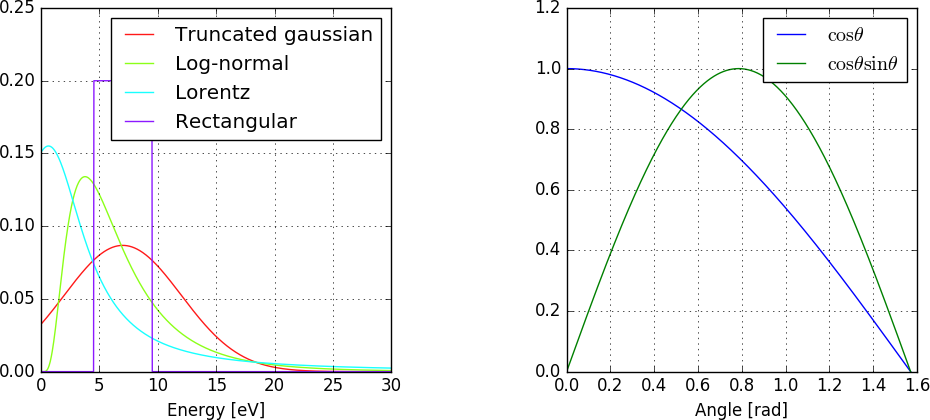
\includegraphics[width=0.8\textwidth]{../plots/distributions.png}
    \caption{
        The left plot shows a cut-off normal distribution characterized by a width and a standard deviation.
        A log-normal distribution with the same mean and variance as the undistorted Gaussian distribution is shown in green.
    The log-normal distribution does not extend to negative values.
    }
    \label{fig:distribution}
\end{figure}


\subsection{Energy of new photoelectrons}

It would be possible to introduce a log-normal distribution for the energy of new macroparticles instead of a truncated Gaussian distribution.
Such a log-normal distribution is also used in the case of new macroparticles from secondary emission multipacting in PyECLOUD.
Alternatively, a truncated Lorentzian is suggested by the results shown in Fig.~\ref{fig:cimino_cu_spectrum}.
Figure~\ref{fig:distribution} visualizes these three approaches.
%For the log-normal distribution, the parameters $\sigma_l$ and $\mu_l$ have to be used in order to achieve the same sample variance and mean as for a normal distribution characterized by $\sigma_n$ and $\mu_n$.
%\begin{align}
%    \sigma_l &= \sqrt{\log\left(\frac{\sigma_n^2}{\mu_n^2}+1\right)}
%    \\
%    \mu_l &= \log\mu_n - \frac{\sigma_l^2}{2}
%\end{align}
A branch called "photoemission" on GitHub adds a new input parameter \textbf{energy\_distribution}, the choices are in addition also a monoenergetic and a rectangular distribution.

\subsection{Delayed photoelectron production}

In PyECLOUD, photoelectrons are generated in parallel to the beam charge.
This means that the difference in path length is not considered.
Until a photon hits the chamber wall, the bunch has moved further due to the bending, see Fig.~\ref{fig:drawing}.
\begin{figure}[tbh]
    \centering
    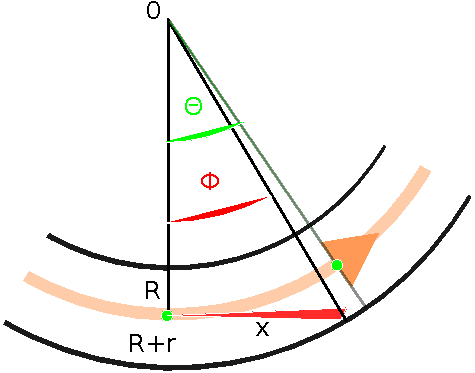
\includegraphics[width=0.5\textwidth]{../scripts/drawing.pdf}
    \caption{The path difference between protons (green) and photons(red).}
    \label{fig:drawing}
\end{figure}
The path difference is calculated in the following way, where $R=2803.95$~m for the LHC, and $r=22$~mm.
$x$ is the distance travelled by the photons before the wall is reached.
\begin{align}
    (R+r)^2 &= R^2 + x^2
    \\
    x &= \sqrt{2Rr + r^2} = 11.1~\text{m}
    \\
    \Phi &= \tan\frac{x}{R} = 0.00396136
    \\
    \Theta &= \frac{x}{R} = 0.00396134
    \\
    \Delta t &= \frac{R(\Theta - \Psi)}{c} = 1.938\cdot10^{-13}~s
\end{align}
This path difference is negligible as it is much smaller than a time step in the simulation, normally around $10^{-11}$~s.

Furthermore, photons that are absorbed only after (multiple) reflections (note that the reflection coefficient for Copper without sawtooth is larger than 80\%) are delayed with respect to the originating beam charge.
One reflection in normal direction leads to a delay of $\Delta t = \frac{2r}{c} = 1.48\cdot10^{-10}$~s, insignificant with respect to the bunch spacing of $2.5\cdot10^{-8}$, but longer than a time step in the simulations.

\subsection{Distribution of photoelectrons in the chamber.}

Another idea would be to simulate the distribution of absorbed photons, and therefore the positions of new electron macroparticles.
Currently, there is only a choice between a cosine and a uniform distribution of $\Psi$ in Fig.~\ref{fig:gt}
Based on the high reflectivity of the non-sawtooth parts of the LHC chamber, a uniform distribution might be the best approximation for the time being.

Figure~\ref{fig:time} visualizes the time a photoelectron with a given energy and emission angle within the e-cloud stripes in a dipole needs to reach the opposing wall in absence of electric fields.
In the currently used photoemission module of PyECLOUD this hardly makes a difference as photoelectrons are created simultaneously with the bunch charge and are therefore immediately accelerated.
In case additional photoelectrons were created independent of time, or delayed with respect to the bunch, it may become relevant as low energy photoelectrons are more relevant because they do not reach the wall before the next proton bunch arrives and cannot get lost.

\begin{figure}[tbh]
    \centering
    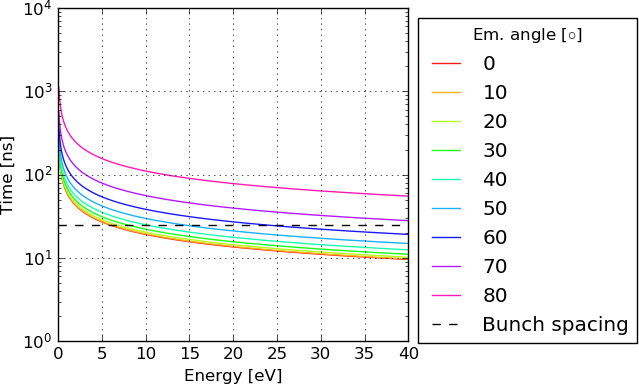
\includegraphics[width=0.55\textwidth]{../plots/time.png}
    \caption{The time needed for a photoelectron in a dipole e-cloud stripe to reach the opposing wall in dependence of the emission angle relative to the surface normal and in absence of electric fields.}
    \label{fig:time}
\end{figure}

